\chapter{Related Work}
\label{RelatedWork}
\section{Neural Networks}
\label{neural_networks}

\overridetextsize
Artificial Intelligence (A.I.), Deep Learning, and Machine Learning have become
buzzwords in recent years, with media, movies, and the general public often
romanticizing and sometimes even humanizing A.I.s. However, what propelled this
enthusiasm is rooted in reality. More recent achievements and revolutions made
in multiple domains with the help of neural networks, even if not rivaling human
capabilities in most scenarios, have been consequent.

The enthusiasm of the general public and scientific community in artificial
intelligence is relatively recent; however, this idea of artificially mimicking
the human brain (seen in figure \ref{fig:biological_neuron}) dates back almost a
century, when a neurophysiologist and a mathematician proposed the first
mathematical model of a neuron (see figure \ref{fig:mccullock_neuron}) called
the McCulloch-Pitts Neuron \cite{warren_s_mcculloch_walter_pitts_logical_1943}.

\begin{figure}[ht]
    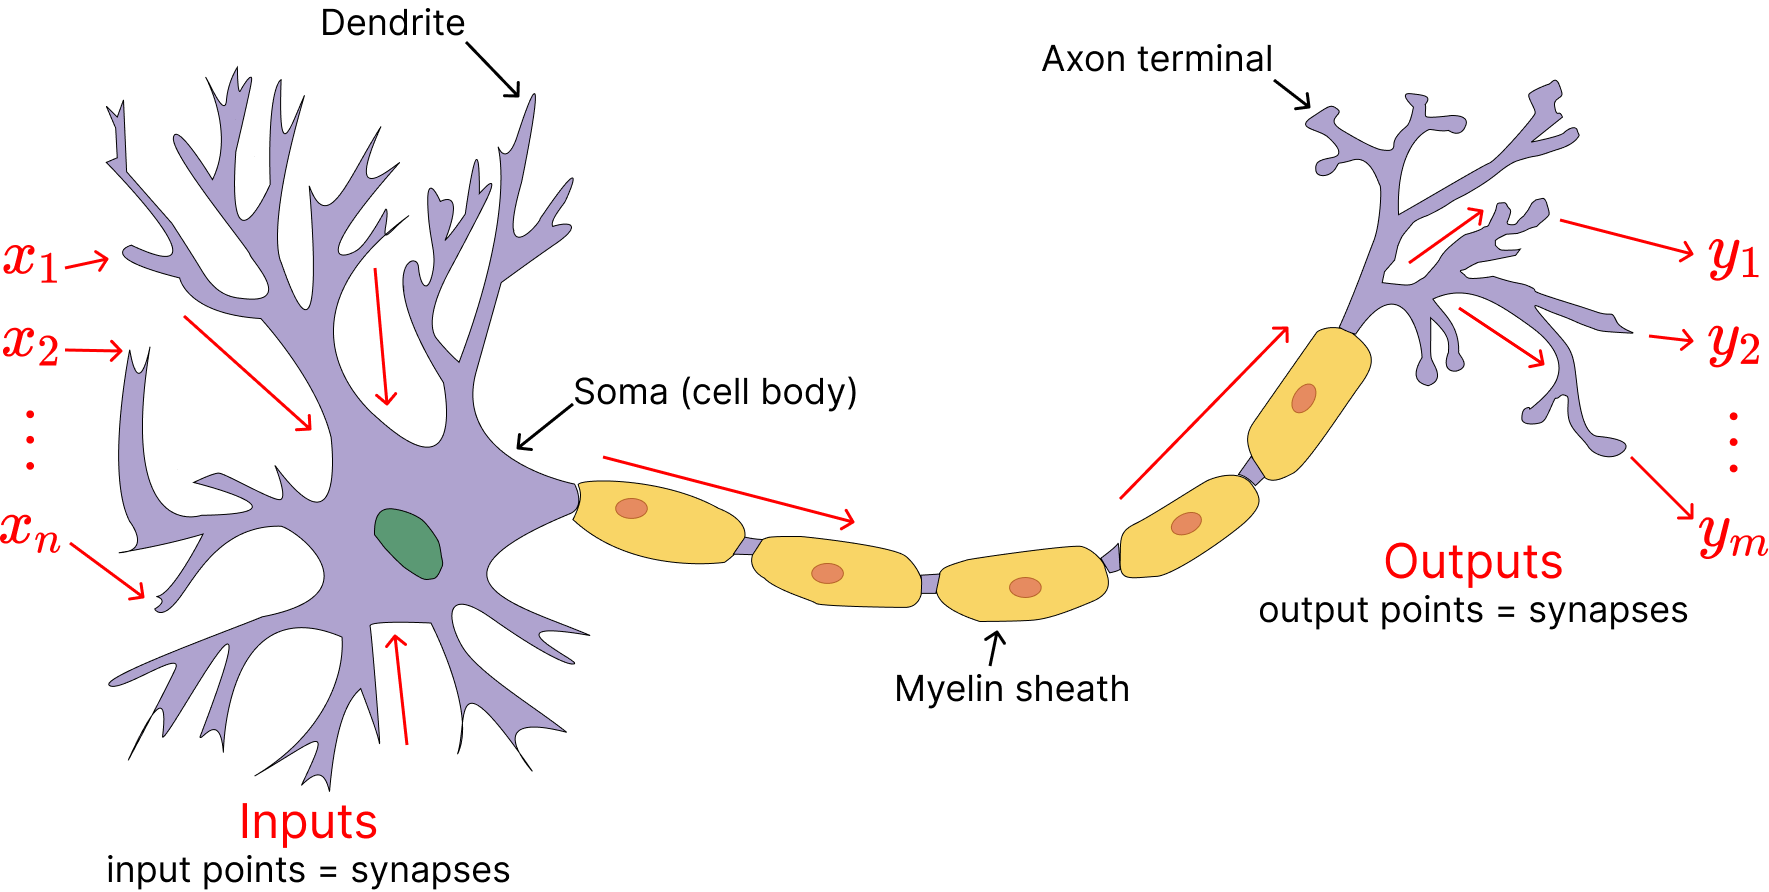
\includegraphics[clip,width=1\columnwidth]{Figures/related/biological_neuron.png}
    \caption{ Representation of a biological neuron. }
    \label{fig:biological_neuron}
\end{figure}

\begin{figure}[htp]
    \centering
    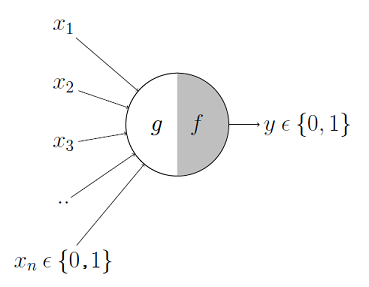
\includegraphics[clip,width=.5\columnwidth]{Figures/related/cullock-neuron.png}
    \caption{ McCulloch-Pitts Neuron, first mathematical model of a neuron. }
    \label{fig:mccullock_neuron}
\end{figure}

Fifteen years later, a psychologist used the McCulloch-Pitts Neuron, where he
proposed the Mark I Perceptron \cite{brain_perceptron_1958}. The breakthrough
proposed by Rosenblatt was that the network could learn by modifying the
neurons' weights through successively passed inputs to minimize the difference
between the desired output and the actual output.

During the next few decades, the field saw some minor improvements, but the
delivery and actual real-world use of A.I.s was minimal, if not nonexistent, and
could not live up to the buildup displayed in media, even at that time. Finally,
M. Minsky published a book that laid out problems with neural networks
\cite{minsky_perceptrons_1969}, notably with their conclusion on the perceptron
proposed by Rosenblatt, stating that this approach could not be translated into
multi-layered neural networks, as the computational cost to evaluate each
layers' neurons would be astronomic. This book, among others, started the era of
"A.I. winter," a period of reduced funding and interest in artificial
intelligence research.

The interest and enthusiasm for neural networks rallied in the nineties with the
rediscoveries of the components that now form the pillar of today's neural
networks: Backprogration and Gradient Descent.


\paragraph{Neural networks,} also known as artificial neural networks (ANNs),
are a subset of machine learning and are at the heart of deep learning
algorithms. Their name and structure are inspired by the human brain, mimicking
the way that biological neurons (see fig. \ref{fig:biological_neuron}) signal to
one another.

Artificial neural networks are thus, similarly to the human brain, comprised of
multiple layers of artificial neurons (see fig. \ref{fig:artificial_neuron} and
fig. \ref{fig:fcnn}).

\begin{figure}[ht]
    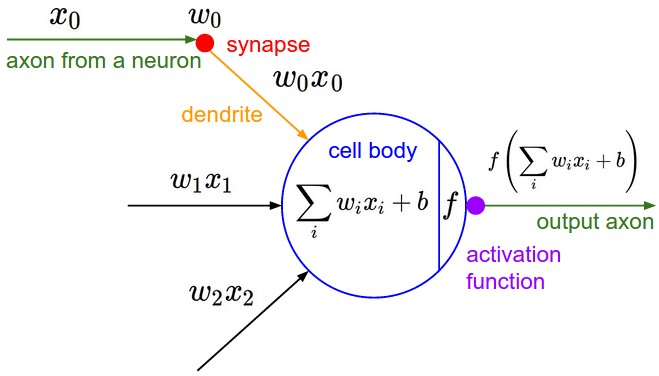
\includegraphics[clip,width=1\columnwidth]{Figures/related/artificial_neuron.jpeg}
    \caption{ Representation of an artificial Neuron. }
    \label{fig:artificial_neuron}
\end{figure}

\begin{figure}[t]
    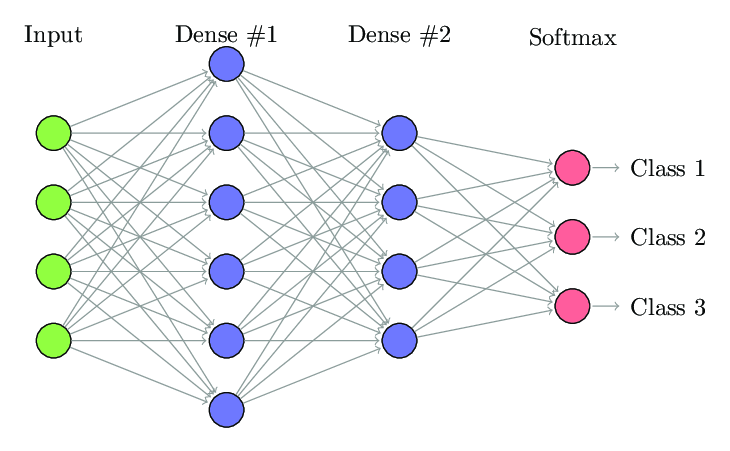
\includegraphics[clip,width=1\columnwidth]{Figures/related/fcnn.png}
    \caption{ Fully connected neural network containing two hidden layers. }
    \label{fig:fcnn}
\end{figure}

% https://www.oreilly.com/library/view/tensorflow-for-deep/9781491980446/ch04.html

Figure \ref{fig:fcnn} represents a simple neural network architecture with two
hidden fully connected layers between the input and output layer. Each hidden
layer contains an arbitrary number of artificial neurons that are fully
connected to the next layer of neurons. The input layer contains several nodes
(or neurons) equal to the dimension of the input. For example, if using a black
and white image of 24 pixels, the input layer would contain $24 \times 24$
nodes. As for the output layer, the number of nodes represents the number of
classes. This type of architecture is widely used. Their primary advantage is
that they are structure agnostic, \emph{i.e.,} no particular assumptions need to
be made about the input.

% https://andrew.gibiansky.com/blog/machine-learning/fully-connected-neural-networks/
Mathematically, we can represent the network shown in figure \ref{fig:fcnn}.

Let $x \in \mathbf{R}$ represents the input. Then, we can perform forward
propagation as follows:

Let $a^{[1]}$ represent the first hidden layer and $a^{[1]}_{i}$ represent
$a^{[1]}$'s $i_{th}$ node:
\begin{equation} \label{eq:fcnn_layer_1}
    A^{[1]} =
    \begin{cases}
        a^{[1]}_{1} = f(x_{1}w^{[1]}_{11} + x_{2}w^{[1]}_{21} + x_{3}w^{[1]}_{31} + x_{4}w^{[1]}_{41} + b^{[1]}_{1}) \\
        a^{[1]}_{2} = f(x_{1}w^{[1]}_{12} + x_{2}w^{[1]}_{22} + x_{3}w^{[1]}_{32} + x_{4}w^{[1]}_{42} + b^{[1]}_{2}) \\
        a^{[1]}_{3} = f(x_{1}w^{[1]}_{13} + x_{2}w^{[1]}_{23} + x_{3}w^{[1]}_{33} + x_{4}w^{[1]}_{43} + b^{[1]}_{3}) \\
        a^{[1]}_{4} = f(x_{1}w^{[1]}_{14} + x_{2}w^{[1]}_{24} + x_{3}w^{[1]}_{34} + x_{4}w^{[1]}_{44} + b^{[1]}_{4}) \\
        a^{[1]}_{5} = f(x_{1}w^{[1]}_{15} + x_{2}w^{[1]}_{25} + x_{3}w^{[1]}_{35} + x_{4}w^{[1]}_{45} + b^{[1]}_{5}) \\
        a^{[1]}_{6} = f(x_{1}w^{[1]}_{16} + x_{2}w^{[1]}_{26} + x_{3}w^{[1]}_{36} + x_{4}w^{[1]}_{46} + b^{[1]}_{6})
    \end{cases}
    ,
\end{equation}
or in vectorized form:
\begin{equation} \label{eq:fcnn_layer_1_vec}
    A^{[1]} = f(W^{[1]} X + b^{[1]}),
\end{equation}
where $b^{[1]}$ represents the bias for the first hidden layer. Biases are
learnable (by the model) parameters used to shift the activation function
(explained next paragraph) right or left, in order to better fit to the data.

Then, from the first hidden layer to the second hidden layer:
\begin{equation} \label{eq:fcnn_layer_2_vec}
    A^{[2]} = f(W^{[2]} A^{[1]} + b^{[2]}),
\end{equation}
where we utilize the output of the previous layer $A^{[1]}$. We can observe the
simplicity of adding or removing a hidden layer from a fully-connected network.

Finally, we can compute the final layer of the network:
\begin{equation} \label{eq:fcnn_layer_last}
    \begin{cases}
        y_{1} = f(a^{[2]}_{1}w^{[3]}_{11} + a^{[2]}_{2}w^{[3]}_{21} + a^{[2]}_{3}w^{[3]}_{31} + a^{[2]}_{4}w^{[3]}_{41} + a^{[2]}_{5}w^{[3]}_{51} + a^{[2]}_{6}w^{[3]}_{61} + b^{[3]}_{1}) \\
        y_{2} = f(a^{[2]}_{2}w^{[3]}_{12} + a^{[2]}_{2}w^{[3]}_{22} + a^{[2]}_{3}w^{[3]}_{32} + a^{[2]}_{4}w^{[3]}_{42} + a^{[2]}_{5}w^{[3]}_{52} + a^{[2]}_{6}w^{[3]}_{62} + b^{[3]}_{2}) \\
        y_{3} = f(a^{[2]}_{3}w^{[3]}_{13} + a^{[2]}_{2}w^{[3]}_{23} + a^{[2]}_{3}w^{[3]}_{33} + a^{[2]}_{4}w^{[3]}_{43} + a^{[2]}_{5}w^{[3]}_{53} + a^{[2]}_{6}w^{[3]}_{63} + b^{[3]}_{3}) \\
    \end{cases}
    ,
\end{equation}
Alternatively, in the vectorized form:
\begin{equation} \label{eq:fcnn_layer_last_vec}
    Y = f(W^{[3]} A^{[2]} + b^{[3]}),
\end{equation}

In the previous equations (Eq. \ref{eq:fcnn_layer_1}, Eq.
\ref{eq:fcnn_layer_1_vec}, Eq. \ref{eq:fcnn_layer_2_vec}, Eq.
\ref{eq:fcnn_layer_last}, Eq. \ref{eq:fcnn_layer_last_vec}), $f$ represents a
nonlinear function, also called activation function. Activation functions act as
the \emph{axon} seen in figure \ref{fig:biological_neuron}. It takes in the
output signal from the previous neuron and converts it into the input for the
next neuron. These nonlinear functions add non-linearity to a neural network, as
their name implies.

\begin{figure}[htb]
    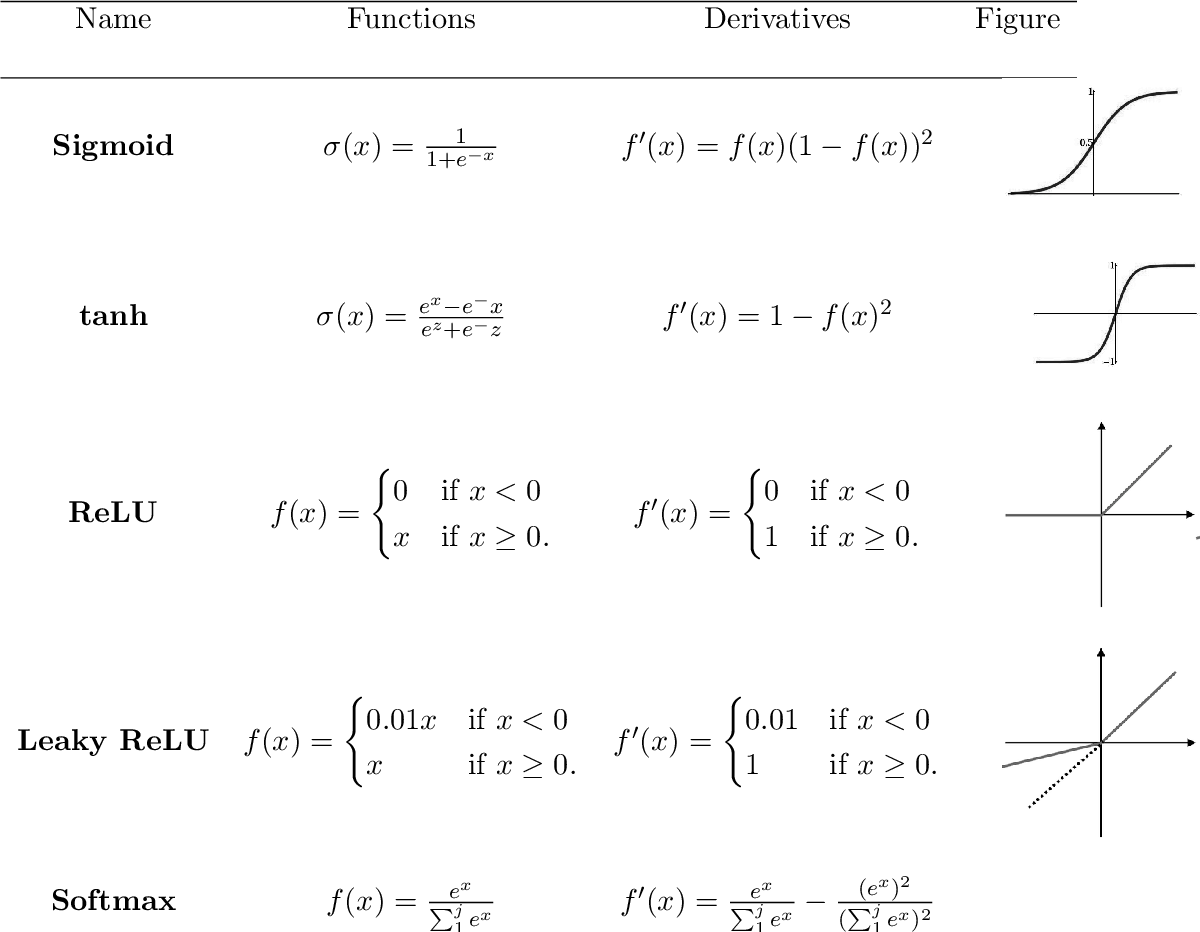
\includegraphics[clip,width=1\columnwidth]{Figures/related/activation_functions.png}
    \caption{ Widely used activation functions. }
    \label{fig:activation_functions}
\end{figure}

Figure \ref{fig:activation_functions} shows some of the widely used activation
functions used in neural networks. In our previous example, the final layer of
our fully connected neural networks contains three nodes (for three
classes); accordingly, this network architecture would be used for multi-class
classification problems. The activation function widely used for this type of
problem is the softmax function, seen in figure \ref{fig:activation_functions}),
where it's equation is:
\begin{equation} \label{eq:softmax}
    f(x) = \frac{e^{x}}{\sum^{j}_{i}e^{x}},
\end{equation}
where $x$ is the input, $j$ is the number of classes and $e$ is the standard
exponential function for output vector.


The softmax function outputs values in the range of 0 to 1. In our neural
network example from figure \ref{fig:fcnn}, with three output classes, the
model's output could be a vector such as: $[0.8, 0.1, 0.1]$. We can translate
this output as the model being 80\% confident about the input being the first
class and 10\% confident for the second and third class, respectively.

As for the hidden layers, a widespread activation is the rectified linear unit,
commonly referred to as ReLU:
\begin{equation} \label{eq:relu}
    f(x) =
    \begin{cases}
        0 \quad \textrm{if} \; x < 0 \\
        x \quad \textrm{if} \; x \geq 1
    \end{cases}
    ,
\end{equation}
or its modification Leaky ReLU:
\begin{equation} \label{eq:leaky_relu}
    f(x) =
    \begin{cases}
        0.01x \quad \textrm{if} \; x < 0 \\
        x \quad \quad \; \; \; \textrm{if} \; x \geq 1
    \end{cases}
    .
\end{equation}
We refer to passing the input through layer-by-layer like evoked beforehand as
"forward propagation." Forward propagation is one of the core processes needed
to train a neural network. Backpropagation \cite{rumelhart_learning_1986} is the
next step in this process, and it refers to the method of calculating the
gradient of the parameters of the neural network, i.e., weights and biases.
Inversely with forward propagation, this method traverses the network from the
output to the input to compute gradient with respect to some parameters. The
objective of updating these parameters is to minimize a chosen cost function.
For example, in our neural network example again, we could use the cross-entropy
function defined as:
\begin{equation} \label{eq:cross-entropy}
    -\sum^{3}_{c=1}y_{o,c} \log{(p_{o,c})},
\end{equation}
for a three-classes classification problem, where $y$ is a binary indicator if
class label $c$ is the correct classification for observation $o$ and $p$ is the
predicted probability that $o$ is of class $c$.

Forward propagation and backpropagation are alternatively used when training a
neural network and are interdependent: forward propagation computes and stores
intermediate variables and parameters, while backpropagation computes the
gradients of these same parameters. Training a network thus requires
considerably more memory than simply predicting a sample, as backpropagation
requires the intermediate values in order to be computed.

To recapitulate, a neural network can be written as a function $F(x)=y$, where
$x$ represents the input and $y$ represents the output. The final layer of a
neural network performing classification is often the softmax activation
function. Therefore, $F(x)$ outputs a probability distribution, where $F(x)_{i}$
represents the probability that input $x$ belongs to class $i$. We write the
final output of the layer as $F(x)=\textup{softmax}(Z(x))$, where $Z(x)$ is the
network output vector containing \textit{logits}, \emph{i.e.,} raw values before
the activation function. Finally, the classifier function that returns the most
likely class label can be written as $C(x)=\textup{argmax}_{i}{(F(x)_{i})}$.

\section{Convolutional Neural Networks}
\label{CNNs}
% https://paperswithcode.com/methods/category/convolutional-neural-networks

\begin{figure}[ht]
    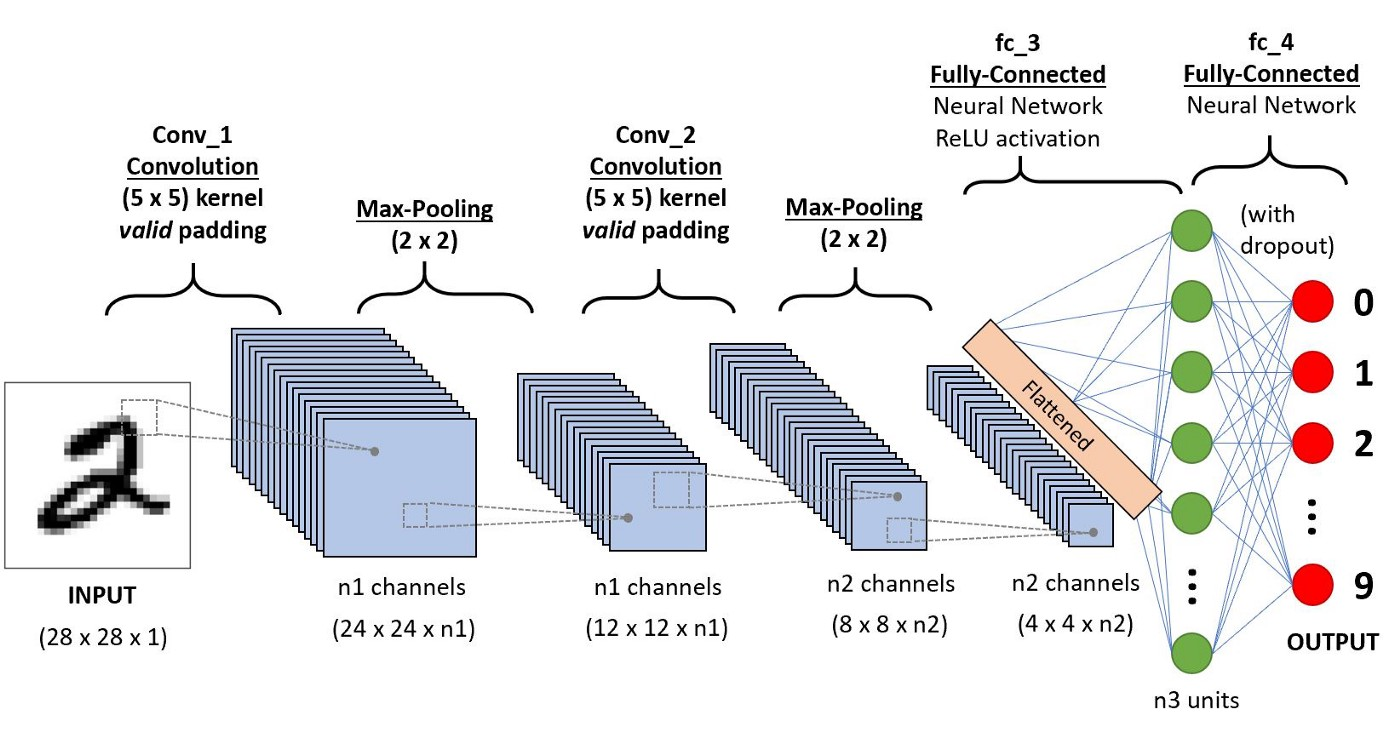
\includegraphics[clip,width=1\columnwidth]{Figures/related/cnn.jpeg}
    \caption{ Architecture of a classic convolutional neural network. }
    \label{fig:cnn}
\end{figure}

Convolutional neural networks (CNNs) \cite{lecun_object_1999}, similarly to the
neural network architectures discussed in the previous section
\ref{neural_networks} are a class of artificial neural networks. CNNs are
commonly used in computer vision to extract features from images or videos and
have been shown to work exceptionally well for this type of data. They are
similarly composed of layers of neurons with learnable parameters, \emph{i.e.,}
weights and biases. The main difference with the more traditional architectures
is that convolutional neural networks make the explicit assumption that the
inputs are of image-type, \emph{i.e.,} images or videos.

The problem with regular neural networks, when applied to images, is that the
fully-connected layers in these architectures do not scale well with this type
of input: a color image of size $224 \times 224$ would represent $150.000$
weights ($224 \times 224 \times 3$), which would quickly result in a costly and
inefficient model. In convolutional neural networks, the neurons are
three-dimensional: width, height, and depth (number of channels: red, green,
blue). These convolutional layers can drastically reduce the number of
parameters, thus the model's size.



Convolutional neural networks, or ConvNets, transform the input image into the
final output vector containing a score for each class through a sequence of
layers. Figure \ref{fig:cnn} shows an example architecture for a convolutional
neural network performing multi-class classification on black and white $28
    \times 28$ images of digits from 0 to 9.

This architecture comports:
\begin{itemize}
    \item Two convolutional layers: the core building block of any ConvNet. Both
          layers contain multiple filters (also called kernels) of size $5
              \times 5$. As seen in figure \ref{fig:kernels}, filters learn visual
          features: the earlier filters, \emph{i.e.,} the ones present at
          shallow depth, learn more basic features. In contrast, filters at the
          last layers learn more complex ones, as seen in figure
          \ref{fig:kernels_5}, since they are combinations of all the previous
          layer's filters.
          \begin{figure}[ht]
              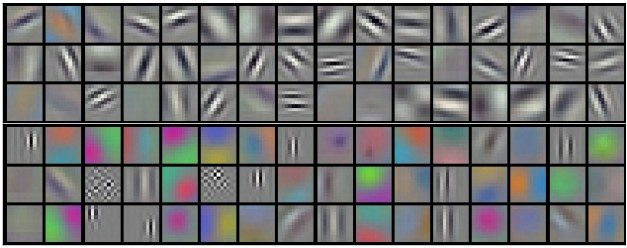
\includegraphics[clip,width=1\columnwidth]{Figures/related/kernels.jpeg}
              \caption{ $11 \times 11 \times 3$ filters learned by the first convolutional
                  layer on $224 \times 224 \times 3$ input images, experiment by
                  \cite{krizhevsky_imagenet_2017-1}. }
              \label{fig:kernels}
          \end{figure}
    \item Pooling layers: these layers will perform a down-sampling operation
          along the spatial dimensions, \emph{e.g.,} width and height. The
          primary function of a pooling layer is to reduce the spatial size of
          the representation, to reduce the number of parameters, thus reducing
          the computation cost of the model.
    \item Fully connected layers: as seen in the previous section
          \ref{neural_networks}. Since neurons from convolutional layers are
          multidimensional, their results need to be flattened before being fed
          into fully-connected layers. This last layer, similarly to ANNs seen
          previously, will output a probability vector containing the score for
          each class.
\end{itemize}



\begin{figure}[htp]
    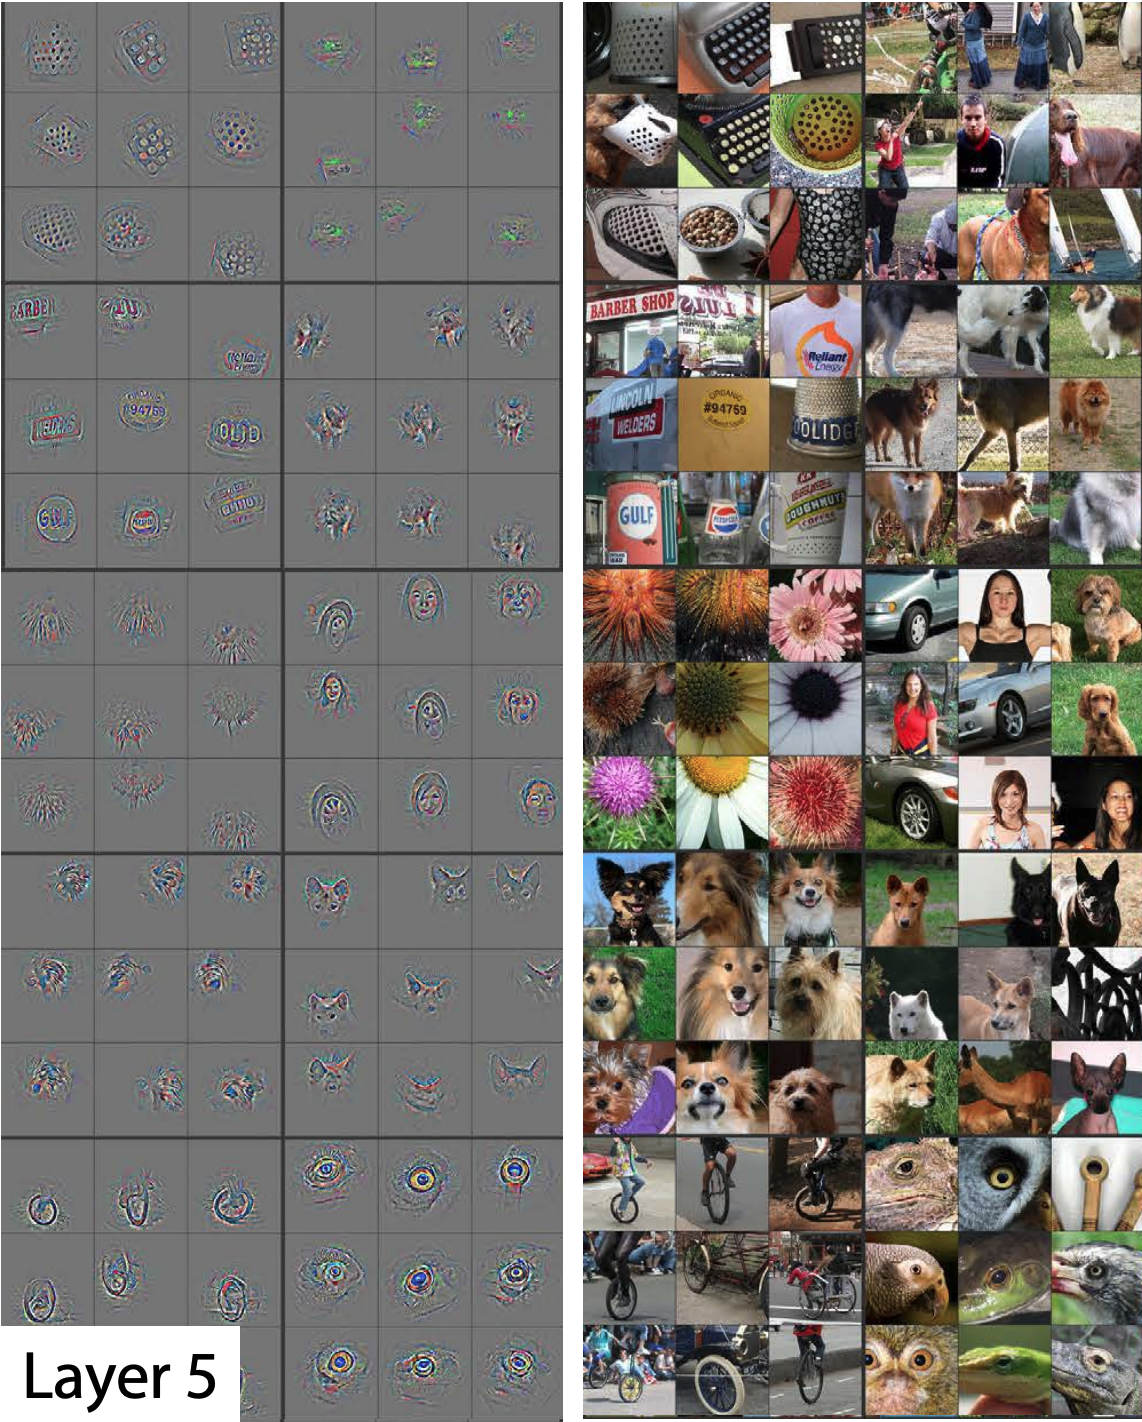
\includegraphics[clip,width=1\columnwidth]{Figures/related/kernels_5.png}
    \caption{ Filters learned by the fifth convolutional layer, experiment by
        \cite{zeiler_visualizing_2013}. }
    \label{fig:kernels_5}
\end{figure}

In short, convolutional neural networks are artificial networks that contain
convolutional layers. These architectures perform exceptionally well on
image-based data with the added benefit of fewer parameters compared to more
traditional ANNs.


In this work, since the entirety of my research is conducted on images,
convolutional neural networks are the only type of architecture that I consider.

\section{Adversarial Examples}
\label{Adversarial_examples}

As seen with figure \ref{fig:adversarial_examples}, adversarial examples are
samples that contain intentional feature modifications that cause a model to
misclassify the sample, \emph{e.g.} an image of a "shark" being misclassified as
a "bee" after adding an invisible (for a human observer) modification to the
image.

A neural network classifying an image of a shark as a bee may only seem comical
and not particularly problematic. However, with the rapidly growing usage of
neural networks in real-world applications, we need to have the certitude that
the models in use will not be as trivially fooled.

\begin{figure}[b]
    \centering
    \subfloat[]{%
        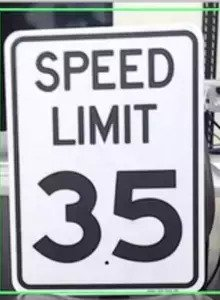
\includegraphics[clip,width=.33\linewidth]{Figures/related/artificial_examples/7.jpeg}%
    } \subfloat[]{%
        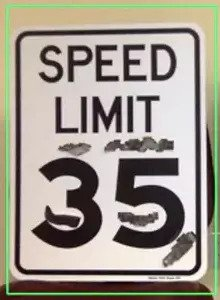
\includegraphics[clip,width=.33\linewidth]{Figures/related/artificial_examples/10.jpeg}%
    } \subfloat[]{%
        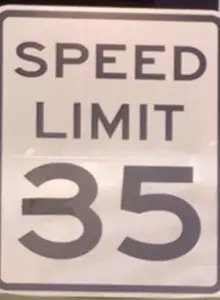
\includegraphics[clip,width=.33\linewidth]{Figures/related/artificial_examples/17.jpeg}%
    } \caption{Speed limit signs modified (B, C) that fools the Tesla model X
        and S (model 2016). (B) is identified as a 45-mph sign, while (C) is
        identified as a 85-mph speed sign.}
    \label{fig:mcafee_tesla}
\end{figure}

Recently, McAfee Advanced Threat Research researchers experimented with
adversarial examples in a physical context \cite{noauthor_model_2020}. They
physically applied modifications to road speed signs in order for a Tesla car to
misidentify the signs. Figure \ref{fig:mcafee_tesla} shows the original 35-mph
road sign (A) as well as two of the physical adversarial examples they created
(B, C). (A) is accurately identified with a 95.93\% confidence, while (B) is
wrongly identified as a 45-mph sign with 99.88\% confidence, and (C) is also
wrongly identified, but as an 85-mph sign! In this context, it is easy to
imagine why and how this can be a problem that needs to be addressed.




With the ever-growing research on the vulnerability of NNs, there are now many
different methods to generate adversarial examples. The common objective of such
methods is to, from a normal image $x$, create a perturbation $\delta$ and add
it to the original image so that the new sample $x^{\prime}=x+\delta$ is
misclassified by a model. We refer to a sample that fulfills this objective as
an \textit{untargeted} adversarial example.

On the contrary, a \textit{targeted} adversarial example $x^{\prime}$ is
designed to be classified by a model as a specified target class $t$. As a
result, targeted adversarial examples are typically more challenging to produce
and may require a more significant perturbation than untargeted attacks.

We can thus formulate the optimization problem to craft adversarial examples as:
\begin{equation} \label{eq:adversarial_example_min}
    \min_{x}D(x+\delta),
\end{equation}


such that the classification $C(x^\prime)\neq{y}$ for an untargeted attack,
where $y$ is the actual class of the input, or $C(x^\prime)={t}$ for a targeted
attack, where $t$ is the targeted class.

$D$ represents a distance metric, usually, $p$-norm defined as:
\begin{equation} \label{eq:p-norm}
    \lVert D
    \lVert_{p}=\left(\sum_{i=1}^{n}|d|^{p}\right)^{\frac{1}{p}}.
\end{equation}

The remainder of this section contains a brief explanation of some of the
popular methods used to generate adversarial examples.

\paragraph{Fast Gradient Sign Method (FGSM).}
Ian Goodfellow \emph{et al} first introduced a method for crafting adversarial examples
\cite{goodfellow_explaining_2015} against GoogLeNet \cite{szegedy_going_2014}.
To generate an adversarial sample $x^{\prime}$ that maximizes the objective $J$,
FGSM uses the gradients of the cost function with respect to the normal input
image $x$:
\begin{align} \label{eq:fgsm} x^{\prime}=x+\epsilon
    sign\left(\nabla_{x}J\left(\Theta,x,y\right)\right),\end{align} where the
multiplier $\epsilon$ is used to ensure that the perturbation is kept small, and
$\Theta$ represents the parameters of the model.

\paragraph{Basic Iterative Method (BIM).}
Alexey Kurakin \emph{et al} proposed an extension of the Fast Gradient Sign Method
\cite{kurakin_adversarial_2017}. Rather than generating the adversarial sample
in one step, BIM applies adversarial noise multiple times with a step size
$\alpha$. The benefit of iteratively crafting the adversarial sample
$x^{\prime}$ is that intermediate results can be clipped at each step to ensure
that the generated samples are within an $\epsilon$ distance to the original
input $x$:
\begin{align} \label{eq:bim}
    x^{\prime}_{n+1}=clip_{x,\epsilon}
    \left\{ x^{\prime}_{n}+\alpha.sign\left(\nabla_{x}J\left(x^{\prime}_{n},y\right)\right)\right\},
\end{align}
where $x^{\prime}_{0}=x$.

\paragraph{Carlini \& Wagner (CW).}
Nicholas Carlini and David Wagner proposed a powerful method to generate
adversarial examples \cite{carlini_towards_2017} that can defeat the defensive
distillation approach published by Nicolas Papernot \emph{et al}
\cite{papernot_distillation_2016}. In their paper, the authors construct an
attack for: $L_{0}$, $L_{2}$ and $L_{\infty}$ distance metrics.

In my experiments, I use the attack that seeks low distortion in the $L_{2}$
distance metric. The final optimization problem for the CW $L_{2}$ attack can be
defined as
\begin{align} \label{eq:cw_min}
    \min{\lVert x^{\prime}-x\lVert_{2}^{2}+c\cdot\ell(x^{\prime})},
\end{align}
where $c$ is a constant chosen via binary search that determine the success
probability of the attack. The loss function $\ell$ is the best among seven
evaluated by the authors, written as
\begin{align} \label{eq:cw_lf}
    \ell(x^{\prime})=\max{\left(\max{\left\{ Z(x^{\prime})_{i}:i\neq t\right\} }-Z(x^{\prime})_{t},-k\right)},
\end{align}
where $-k$ is a parameter to specify how confident we want the adversarial
example to be classified as $t$ by the model.

The CW method is a state-of-the-art attack and effectively finds adversarial
examples with a small perturbation size. However, this method is computationally
expensive to run.

\paragraph{Decoupled Direction and Norm (DDN).}
Jérôme Rony \emph{et al} proposed an improvement over the CW method
\cite{rony_decoupling_2019}. The DDN method can obtain comparable results in
terms of perturbation size but with considerably fewer iterations. At each
iteration $k$, refine noise $\beta_{k}$ by considering a larger norm
$\epsilon_{k+1}=(1+\gamma)\epsilon_{k}$ or smaller norm
$\epsilon_{k+1}=(1-\gamma)\epsilon_{k}$ depending on if $x+\beta_{k}$ is
adversarial or not. Finally, the method returns the clipped adversarial sample
that has the lowest $L_{2}$-norm.

Figure \ref{fig:samples_ae} shows three samples generated using the basic
iterative method (B), decoupled direction and norm (D), and the Carlini \&
Wagner method (F). The model correctly predicts the natural image (A) as an
image of a church while predicting the generated samples as images of chickens.
The perturbation size for each sample is: $L_2 \approx 2.00$ for the BIM sample
(B), $L_2 \approx 1.40$ for the DDN (D) sample and $L_2 \approx 1.37$ for the CW
sample. As discussed earlier, DDN and CW methods can generate samples with a
smaller perturbation than methods such as BIM or FGSM.

\begin{figure}[htb]
    \centering
    \begin{tabular}{@{}cc@{}} \multicolumn{2}{c}{
            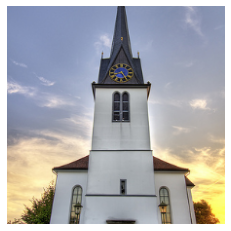
\includegraphics[width=.25\columnwidth]{Figures/related/attacks/original.png}
        }                       \\
        \multicolumn{2}{c}{ (A) Original image }
        \\
        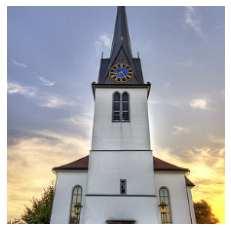
\includegraphics[width=.32\columnwidth]{Figures/related/attacks/bim_1_chicken.png}
                &
        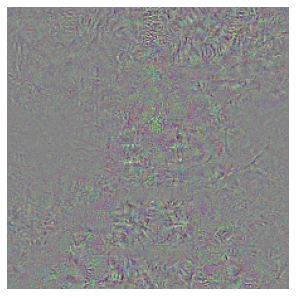
\includegraphics[width=.32\columnwidth]{Figures/related/attacks/bim_1_chicken_diff2.png}
        \\
        (B) BIM & (C) $(B - A)$ \\
        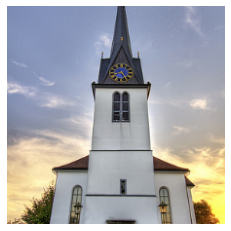
\includegraphics[width=.32\columnwidth]{Figures/related/attacks/ddn_0.85_chicken.png}
                &
        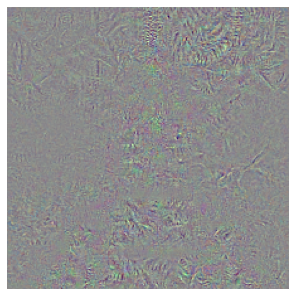
\includegraphics[width=.32\columnwidth]{Figures/related/attacks/ddn_0.85_chicken_diff2.png}
        \\
        (D) DDN & (E) $(D - A)$ \\
        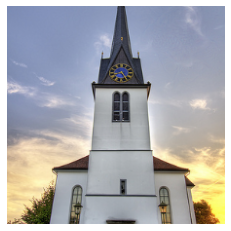
\includegraphics[width=.32\columnwidth]{Figures/related/attacks/cw_0.62_chicken.png}
                &
        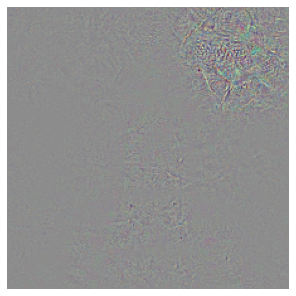
\includegraphics[width=.32\columnwidth]{Figures/related/attacks/cw_0.62_chicken_diff2.png}
        \\
        (F) CW  & (G) $(F - A)$
    \end{tabular}
    \caption{ Adversarial examples generated with different methods. The
        original input image (A) is correctly classified as a "church", while
        all the generated samples: (B), (D) and (F) are identified as a
        "chicken" by the model. }
    \label{fig:samples_ae}
\end{figure}

\clearpage


%---------------------------------------------------------------------
\section{Defending Against Adversarial Examples}
\label{sec:defending_adgainst_adversarial_examples}

Since Christian Szegedy \emph{et al} \cite{szegedy_intriguing_2014} discovered
the existence of adversarial examples, much research has been conducted from the
perspectives of both the attacker, \emph{i.e.,} the party trying to exploit
vulnerabilities in a model and the defending party trying to mitigate these
attacks. The authors also hypothesized that adversarial examples exist due to
the high non-linearity nature of NNs. However, this hypothesis was later
rebutted by Goodfellow \emph{et al} when they argued that adversarial examples
exist due to NNs being too linear rather than the contrary
\cite{goodfellow_explaining_2015}.

The research first focused on defending against adversarial examples by
improving the robustness of neural networks via, among others, adversarial
training \cite{goodfellow_explaining_2015,papernot_limitations_2015}, where
adversarial examples are included in a dataset alongside natural images in order
to train a CNN on both natural images and adversarial samples. The computational
cost required to generate adversarial examples makes this defense approach
computationally expensive, even when using techniques such as FGSM that require
\emph{considerably} less computational work than methods such as CW which can
require hours to generate a single sample on a low-end gpu.

\textit{Defensive distillation} \cite{papernot_distillation_2016} is another
technique to improve the robustness of NN and involves the use of two networks.
A first network $F$ is conventionally trained on inputs $X$ and labels $Y$ and
outputs a probability vector predictions $F(X)$. The second network $F_{d}$ is
then trained on the same inputs $X$, but the labels are replaced by the output
of the first network $F(X)$ as a way of restraining the model from over-fitting
on the data. Defensive distillation is a very effective defense but was defeated
by the more recent CW attack.

Due to the difficulty and computational cost of training robust neural networks
against adversarial examples, recent research has focused on detecting them
instead. However, a recent survey by N. Carlini and D. Wagner examined ten
detection defenses that they all bypassed using their attack method and
concluded that adversarial examples are significantly more complex to detect
than previously recognized \cite{carlini_adversarial_2017}. Furthermore, among
the ten detection methods surveyed, they concluded that only \textit{bayesian
neural network uncertainty} \cite{feinman_detecting_2017} was effective and made
generating adversarial examples nearly five times more difficult on the dataset
CIFAR-10. For their method, Reuben Feinman \emph{et al} use dropout
\cite{srivastava_dropout_2014} to induce randomness during inference and predict
an input multiple times in order to measure the prediction uncertainty. They
show that the prediction uncertainty is typically higher on adversarial examples
compared to normal and noisy images.

\section{Detection Evaluation Metrics}
To attest to the effectiveness of the detection performances of the method
proposed in a later section, I adopt the recall and precision rates defined as
\begin{align} \label{eq:recall}
    recall=\frac{tp}{tp+fn},
\end{align}
where $tp$ (\textit{true positive}) is the number of correctly detected
adversarial examples and $fn$ (\textit{false negative}) is the number of
adversarial examples that are not detected.
\begin{align} \label{eq:precision}
    precision=\frac{tp}{tp+fp},
\end{align}
where $fp$ (\textit{false positive}) is the number of normal images that are
incorrectly identified as adversarial examples.

Finally, we use the $F_{\beta}$ score defined as:
\begin{align} \label{eq:fb}
    F_{\beta}=(1+\beta^{2})\frac{recall\cdot
        precision}{recall+(\beta^{2}precision)},
\end{align}
where $\beta=2$ to emphasize on the recall rate.
